\documentclass[letterpaper]{article}
\usepackage[margin=1in]{geometry} % US Letter with 1-inch margins
\usepackage{tikz}
\usepackage{aeguill}

\begin{document}

\begin{center}
\resizebox{\textwidth}{!}{% scale diagram to fit page width
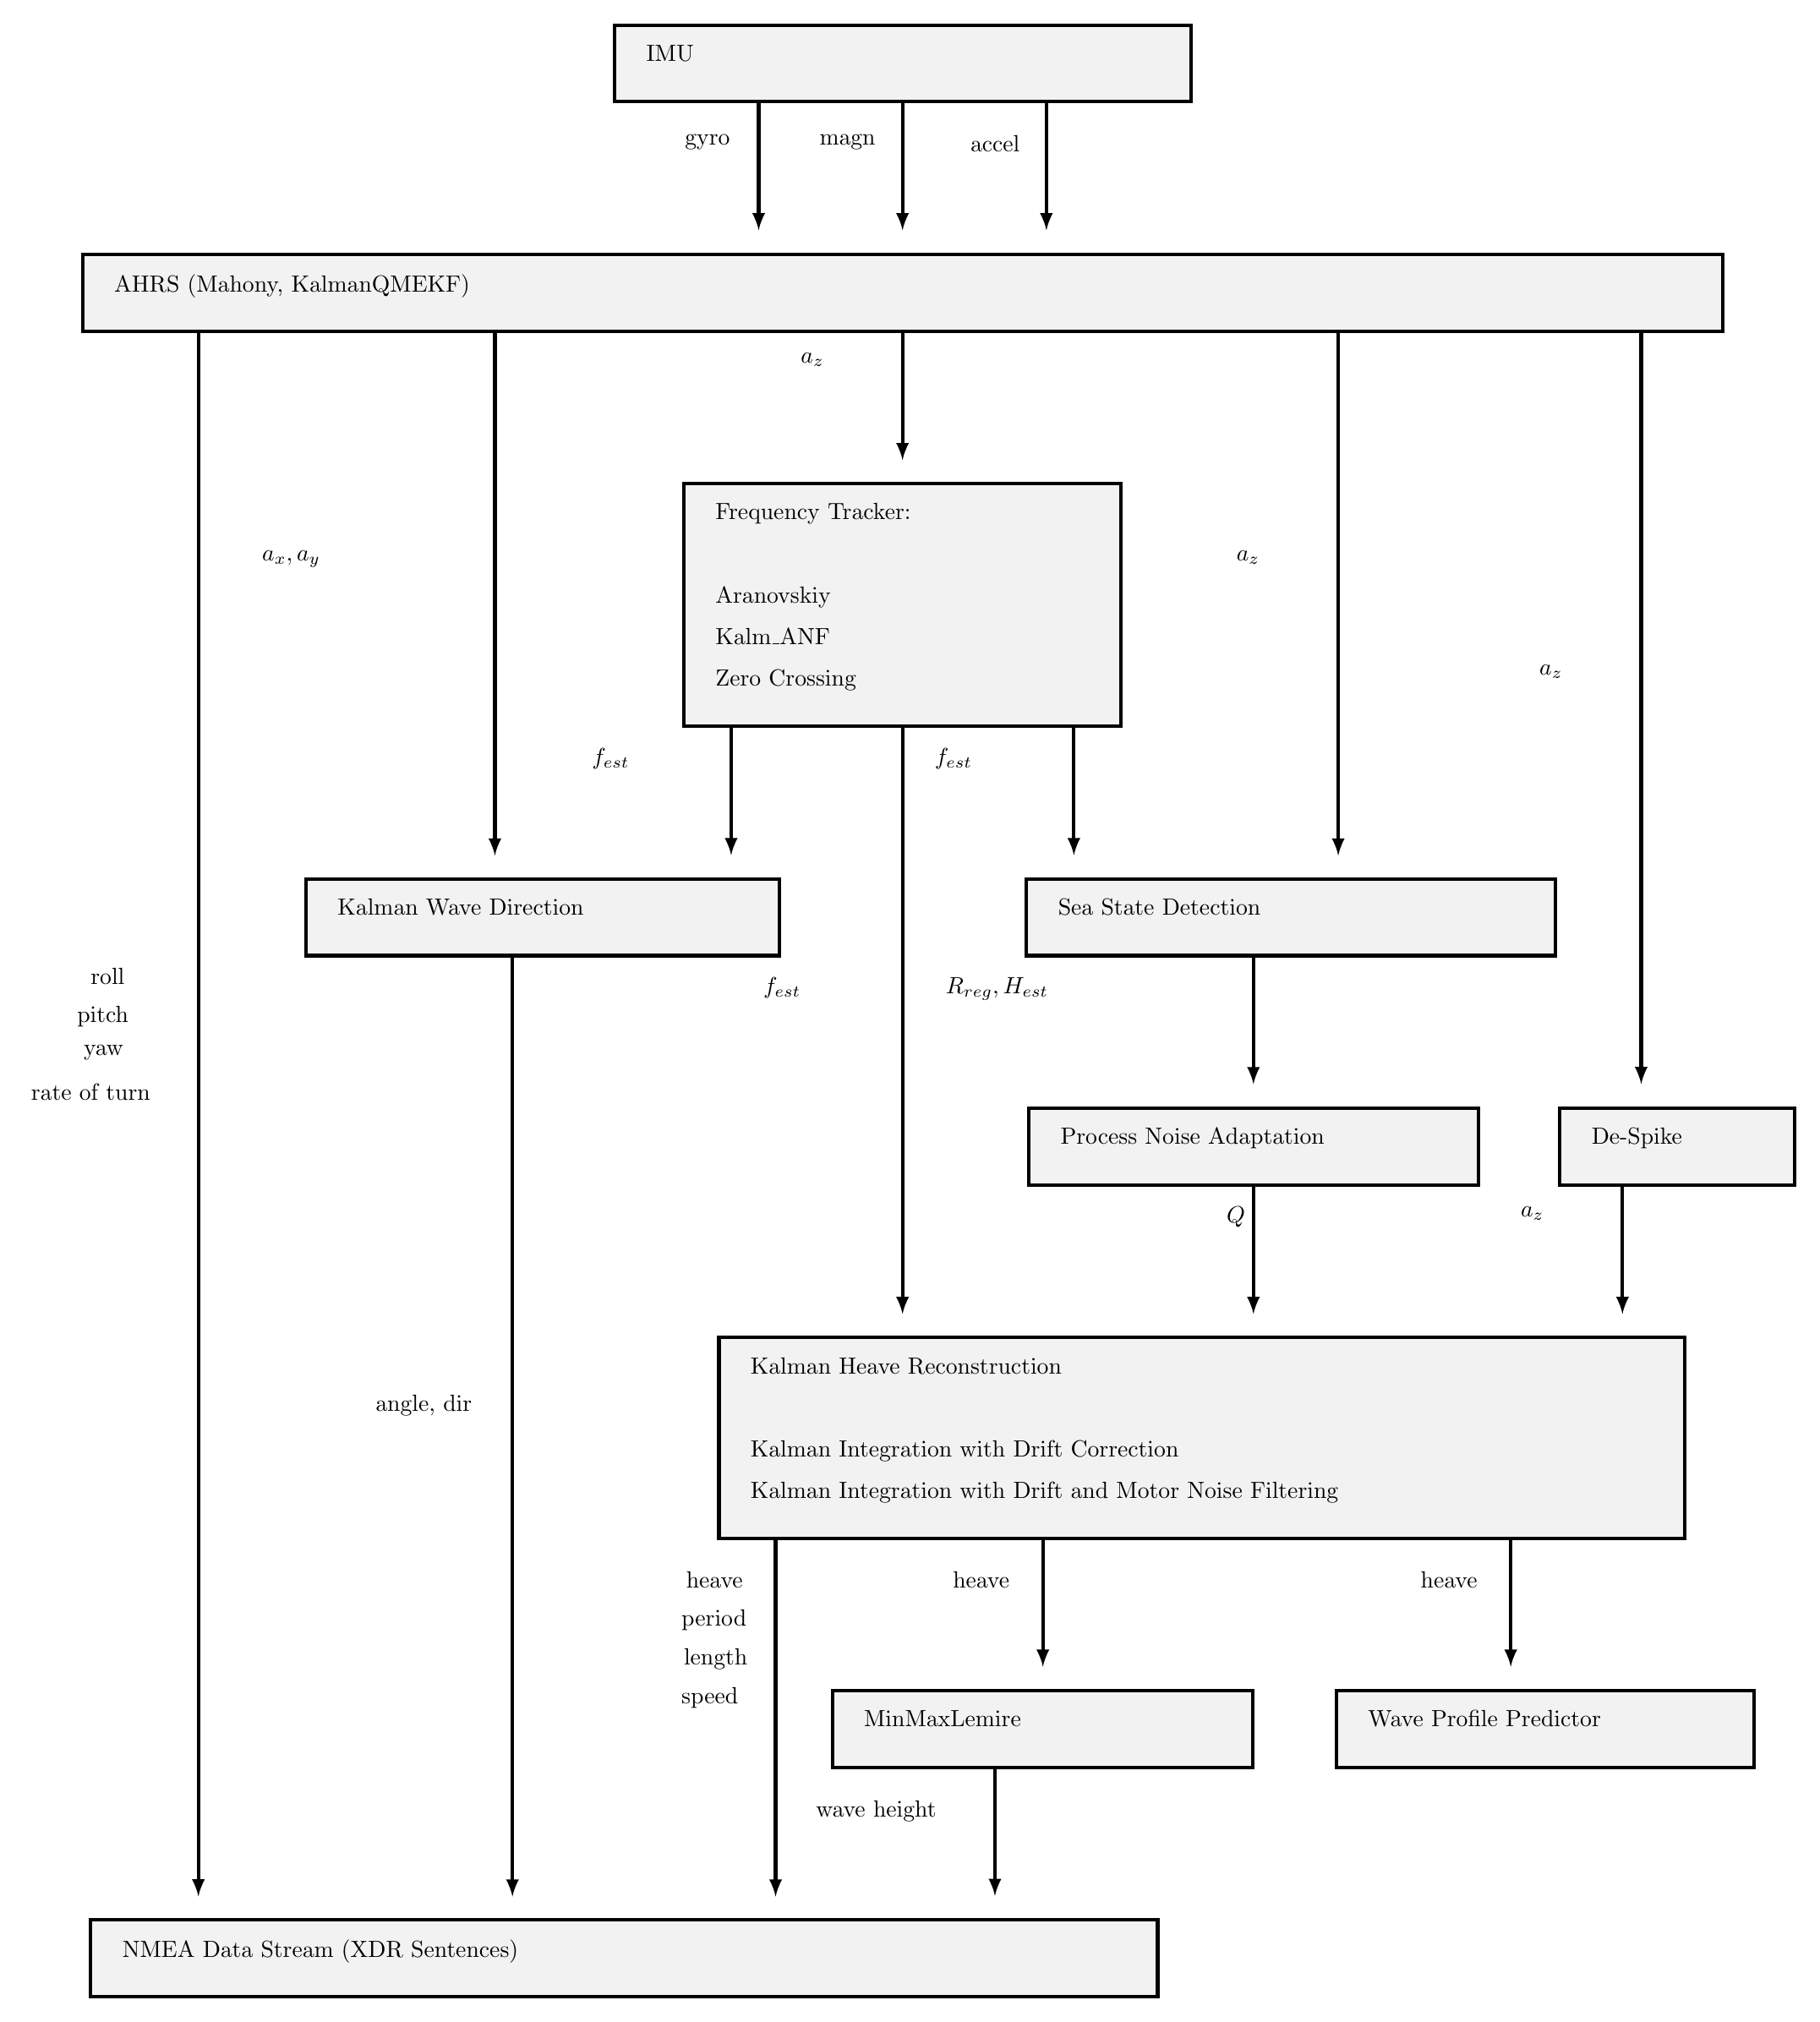
\begin{tikzpicture}[yscale=-1
  ,pstyle0/.style={color=black,fill=gray!10,line width=1.5pt}
  ,pstyle1/.style={color=black,line width=1.5pt}
  ,pstyle2/.style={color=black,fill=black,line width=1.5pt}
]

% --- Rectangles with sharp corners ---
\draw[pstyle0] (260pt,12pt) rectangle (506.2609pt,44.7461pt);
\node at (270pt,17pt)[below right,color=black]{IMU};

\draw[pstyle0] (32.5pt,110pt) rectangle (733.5667pt,142.7461pt);
\node at (42.5pt,115pt)[below right,color=black]{AHRS (Mahony, KalmanQMEKF)};

\draw[pstyle0] (289.5pt,208pt) rectangle (476.3973pt,311.7305pt);
\node at (299.5pt,213pt)[below right,color=black]{Frequency Tracker:};
\node at (299.5pt,248.4922pt)[below right,color=black]{Aranovskiy};
\node at (299.5pt,266.2383pt)[below right,color=black]{Kalm\_ANF};
\node at (299.5pt,283.9844pt)[below right,color=black]{Zero Crossing};

\draw[pstyle0] (128pt,377pt) rectangle (330.3595pt,409.7461pt);
\node at (138pt,382pt)[below right,color=black]{Kalman Wave Direction};

\draw[pstyle0] (436pt,377pt) rectangle (661.9957pt,409.7461pt);
\node at (446pt,382pt)[below right,color=black]{Sea State Detection};

\draw[pstyle0] (304.5pt,573pt) rectangle (717.4414pt,658.9844pt);
\node at (314.5pt,578pt)[below right,color=black]{Kalman Heave Reconstruction};
\node at (314.5pt,613.4922pt)[below right,color=black]{Kalman Integration with Drift Correction};
\node at (314.5pt,631.2383pt)[below right,color=black]{Kalman Integration with Drift and Motor Noise Filtering};

\draw[pstyle0] (437pt,475pt) rectangle (629.2069pt,507.7461pt);
\node at (447pt,480pt)[below right,color=black]{Process Noise Adaptation};

\draw[pstyle0] (36pt,822pt) rectangle (492.0642pt,854.7461pt);
\node at (46pt,827pt)[below right,color=black]{NMEA Data Stream (XDR Sentences)};

\draw[pstyle0] (353pt,724pt) rectangle (532.6658pt,756.7461pt);
\node at (363pt,729pt)[below right,color=black]{MinMaxLemire};

\draw[pstyle0] (664pt,475pt) rectangle (764.4pt,507.7461pt);
\node at (674pt,480pt)[below right,color=black]{De-Spike};

\draw[pstyle0] (568.5pt,724pt) rectangle (747.119pt,756.7461pt);
\node at (578.5pt,729pt)[below right,color=black]{Wave Profile Predictor};

% --- Straight arrows instead of curves ---
\draw[pstyle1,-latex] (444.5pt,45.36pt) -- (444.5pt,99.68pt);
\node at (408.5pt,55.52pt)[below right,color=black]{accel};

\draw[pstyle1,-latex] (321.5pt,45.36pt) -- (321.5pt,99.68pt);
\node at (286.5pt,55.52pt)[below right,color=black]{gyro};

\draw[pstyle1,-latex] (383pt,45.36pt) -- (383pt,99.68pt);
\node at (344pt,55.52pt)[below right,color=black]{magn};

\draw[pstyle1,-latex] (383pt,143.13pt) -- (383pt,197.93pt);
\node at (336pt,148.53pt)[below right]{${a_{z}}$};

\draw[pstyle1,-latex] (456.25pt,312.18pt) -- (456.25pt,366.82pt);
\node at (393.25pt,317.5pt)[below right]{${f_{est}}$};

\draw[pstyle1,-latex] (569.25pt,143.2pt) -- (569.25pt,366.97pt);
\node at (522.25pt,233.09pt)[below right]{${a_{z}}$};

\draw[pstyle1,-latex] (208.75pt,143.2pt) -- (208.75pt,366.97pt);
\node at (105.75pt,233.09pt)[below right]{${a_{x}, a_{y}}$};

\draw[pstyle1,-latex] (309.75pt,312.18pt) -- (309.75pt,366.82pt);
\node at (246.75pt,317.5pt)[below right]{${f_{est}}$};

\draw[pstyle1,-latex] (533pt,410.36pt) -- (533pt,464.68pt);
\node at (398pt,415.52pt)[below right]{${R_{reg}, H_{est}}$};

\draw[pstyle1,-latex] (383pt,312.34pt) -- (383pt,562.93pt);
\node at (320pt,415.64pt)[below right]{${f_{est}}$};

\draw[pstyle1,-latex] (533pt,508.18pt) -- (533pt,562.92pt);
\node at (518pt,513.55pt)[below right]{${Q}$};

\draw[pstyle1,-latex] (698.75pt,143.11pt) -- (698.75pt,464.64pt);
\node at (651.75pt,281.87pt)[below right]{${a_{z}}$};

\draw[pstyle1,-latex] (690.75pt,508.18pt) -- (690.75pt,562.92pt);
\node at (643.75pt,513.55pt)[below right]{${a_{z}}$};

\draw[pstyle1,-latex] (443pt,659.15pt) -- (443pt,713.71pt);
\node at (401pt,669.43pt)[below right,color=black]{heave};

\draw[pstyle1,-latex] (643pt,659.15pt) -- (643pt,713.71pt);
\node at (601pt,669.43pt)[below right,color=black]{heave};

\draw[pstyle1,-latex] (216.25pt,410.12pt) -- (216.25pt,811.95pt);
\node at (154.25pt,594.04pt)[below right,color=black]{angle, dir};

\draw[pstyle1,-latex] (422.5pt,757.36pt) -- (422.5pt,811.68pt);
\node at (342.5pt,767.52pt)[below right,color=black]{wave height};

\draw[pstyle1,-latex] (328.75pt,659.06pt) -- (328.75pt,811.97pt);
\node at (287pt,669.51pt)[below right,color=black]{heave};
\node at (285pt,685.99pt)[below right,color=black]{period};
\node at (286pt,702.47pt)[below right,color=black]{length};
\node at (285pt,718.95pt)[below right,color=black]{speed};

\draw[pstyle1,-latex] (82pt,143.04pt) -- (82pt,811.9pt);
\node at (32.45pt,411.47pt)[below right,color=black]{roll};
\node at (26.68pt,427.95pt)[below right,color=black]{pitch};
\node at (29.47pt,444.43pt)[below right,color=black]{yaw};
\node at (7pt,460.91pt)[below right,color=black]{rate of turn};

\end{tikzpicture}
}% end resizebox
\end{center}

\end{document}
